\documentclass[a4paper,12pt]{article}
\usepackage{amsmath}
\usepackage[margin=0.9in]{geometry}
\usepackage{braket}
\usepackage{graphicx}
\begin{document}
\subsection*{Exercise 10.1}
Let $\ket{\psi}=a\ket{0}+b\ket{1}$ and the initial state be $\ket{\psi_0}=a\ket{000}+b\ket{100}$.\\
Applying a CNOT to the first two qubits we get,\\
$\ket{\psi_1}=a\ket{000}+b\ket{110}$\\
Applying a CNOT to the first and last qubits we get,\\
$\ket{\psi_2}=a\ket{000}+b\ket{111}$
\subsection*{Exercise 10.2}
$P_\pm=\frac{1}{2}(\ket{0}\pm\ket{1})(\bra{0}\pm\bra{1})=
\frac{1}{2}(\ket{0}\bra{0}+\ket{1}\bra{1}\pm\ket{1}\bra{0}\pm\ket{0}\bra{1})
=\frac{1}{2}(I\pm X)$\\
Therefore,\\
$\mathcal{E}(\rho)=(1-2p)\rho+2pP_+\rho P_++2pP_-\rho P_-=
(1-2p)\rho+\frac{1}{2}p(I+X)\rho(I+X)+\frac{1}{2}p(I-X)\rho(I-X)=
(1-2p)\rho+p\rho+pX\rho X=(1-p)\rho+pX\rho X$
\subsection*{Exercise 10.3}
$Z_2Z_3Z_1Z_2=[I\otimes (\ket{00}\bra{00}+\ket{11}\bra{11})-I\otimes (\ket{01}\bra{01}+\ket{10}\bra{10})]
[(\ket{00}\bra{00}+\ket{11}\bra{11})\otimes I-(\ket{01}\bra{01}+\ket{10}\bra{10})\otimes I]=
\underbrace{\ket{000}\bra{000}+\ket{111}\bra{111}}_{P_0}
-(\underbrace{\ket{100}\bra{100}+\ket{011}\bra{011}}_{P_1})\\
+\underbrace{\ket{010}\bra{010}+\ket{101}\bra{101}}_{P_2}
-(\underbrace{\ket{001}\bra{001}+\ket{110}\bra{110}}_{P_3})$
\subsection*{Exercise 10.4}
1)$\ket{000}\bra{000}$, $\ket{111}\bra{111}$: no bit flip\\
$\ket{100}\bra{100}$, $\ket{011}\bra{011}$: first bit flipped\\
$\ket{010}\bra{010}$, $\ket{101}\bra{101}$: second bit flipped\\
$\ket{001}\bra{001}$, $\ket{110}\bra{110}$: third bit flipped\\
2) If our state is $\ket{\psi}=a\ket{000}+b\ket{111}$, then the measurement will
collapse the state into $\ket{000}$ or $\ket{111}$ with probabilities $|a|^2$ or $|b|^2$,
respectively. Hence, only the computational basis states $\ket{000}$ and $\ket{111}$ can 
be corrected.\\
3)Assuming the initial state is $\ket{000}$ the probability that one or fewer bit flips occur is $(1-p)^3+p(1-p)^2$, hence
$F\geq\sqrt{(1-p)^3+p(1-p)^2}$.
\subsection*{Exercise 10.5}
Assuming no more than one error has occurred, $X_1X_2X_3X_4X_5X_6$ will be $1$ if no phase flip occurred
and $-1$ and if one occurred on the first or second block. Identically for $X_4X_5X_6X_7X_8X_9$.
Hence, if both give $-1$ the error is on the second block, otherwise it's on the first block if
$X_1X_2X_3X_4X_5X_6$ gives $-1$ and on the third block if $X_4X_5X_6X_7X_8X_9$ gives $-1$.
If both give $1$ then no error has occurred.
\subsection*{Exercise 10.6}
The eigenvalues of $Z$ are $\pm 1$, hence\\
$Z_1Z_2Z_3(\ket{000}-\ket{111})=\ket{000}-(-1)^3\ket{111}=\ket{000}+\ket{111}$
\subsection*{Exercise 10.7}
Need to prove that $PE_i^\dagger E_jP=\alpha_{ij}P$. $I$ and $X$ are Hermitian, hence suffices
to show for $IX_1$,$II$,$X_1X_1$ and $X_1X_2$.\\
$P\sqrt{(1-p)^3}I\sqrt{p(1-p)^2}X_1P=(1-p)^2\sqrt{p(1-p)}
(\ket{000}\bra{000}+\ket{111}\bra{111})X_1(\ket{000}\bra{000}+\ket{111}\bra{111})=
(1-p)^2\sqrt{p(1-p)}
(\ket{000}\bra{000}+\ket{111}\bra{111})(\ket{100}\bra{000}+\ket{011}\bra{111})=0$\\
$P\sqrt{(1-p)^3}I\sqrt{(1-p)^3}IP=(1-p)^3PP=(1-p)^3P$\\
$P\sqrt{p(1-p)^2}X_1\sqrt{p(1-p)^2}X_1P=p(1-p)^2PIP=p(1-p)^2P$\\
$P\sqrt{p(1-p)^2}X_1\sqrt{p(1-p)^2}X_2=p(1-p)^2
(\ket{000}\bra{000}+\ket{111}\bra{111})(\ket{110}\bra{000}+\ket{001}\bra{111})=0$\\
Hence, the quantum error-correction conditions are satisfied.
\subsection*{Exercise 10.8}
$P=\ket{+++}\bra{+++}+\ket{---}\bra{---}$, hence like in the previous exercise.\\
$PE_i^\dagger E_jP=0$, $i\neq j$\\
$PE_i^\dagger E_jP=P$, $i=j$\\
Hence, the quantum error-correction conditions are satisfied.
\subsection*{Exercise 10.9}
$PIIP=P$\\
$PIP_1P=(\ket{+++}\bra{+++}+\ket{---}\bra{---})(\ket{0}\bra{0}\otimes I\otimes I)
(\ket{+++}\bra{+++}+\ket{---}\bra{---})=
(\ket{+++}\bra{+++}+\ket{---}\bra{---})\frac{1}{\sqrt{2}}(\ket{0++}\bra{+++}+\ket{0--}\bra{---})=
\frac{1}{2}(\ket{+++}\bra{+++}+\ket{---}\bra{---})=\frac{1}{2}P$\\
Identically,\\
$PIQ_1P=\frac{1}{2}P$\\
$PP_1Q_1=0$\\
$PP_1P_1P=PP_1P=\frac{1}{2}P$\\
$PQ_1Q_1P=PQ_1P=\frac{1}{2}P$\\
$PP_1P_2P=(\ket{+++}\bra{+++}+\ket{---}\bra{---})(\ket{0}\bra{0}\otimes \ket{0}\bra{0}\otimes I)
(\ket{+++}\bra{+++}+\ket{---}\bra{---})=
(\ket{+++}\bra{+++}+\ket{---}\bra{---})\frac{1}{2}(\ket{00+}\bra{+++}+\ket{00-}\bra{---})=
\frac{1}{4}(\ket{+++}\bra{+++}+\ket{---}\bra{---})=\frac{1}{4}P$\\
$PP_1Q_2P=(\ket{+++}\bra{+++}+\ket{---}\bra{---})(\ket{0}\bra{0}\otimes \ket{1}\bra{1}\otimes I)
(\ket{+++}\bra{+++}+\ket{---}\bra{---})=
(\ket{+++}\bra{+++}+\ket{---}\bra{---})\frac{1}{2}(\ket{01+}\bra{+++}-\ket{01-}\bra{---})
=\frac{1}{4}(\ket{+++}\bra{+++}+\ket{---}\bra{---})=\frac{1}{4}P$\\
Hence, the quantum error-correction conditions are satisfied.
\subsection*{Exercise 10.10}
$P=\ket{0_L}\bra{0_L}+\ket{1_L}\bra{1_L}$\\
Due to phase and bit flips,\\
$PIX_iP=PIY_iP=PIZ_iP=0$\\
$PIIP=PX_iX_iP=PY_iY_iP=PZ_iZ_iP=P$\\
The $X_i$ and $Y_i$ change the individual qubits, hence if $i\neq j$ $PX_iY_jP=0$, e.g.
for $PX_1Y_2P$ looking at the first triplet, we have\\
$(\bra{000}+\bra{111})i(\ket{110}-\ket{001})=0$\\
$X_iY_i=iZ_i$, hence $PX_iY_iP=0$\\
For $Z_iZ_j$ if $i$ and $j$ belong to different triplets then we have a phase flip on $2$
separate triplets, hence $PZ_iZ_jP=0$. \\
However, if $i$ and $j$ are in the same triplet, then
we apply $2$ phase shifts to the triplet which is equivalent to no change, hence
$PZ_iZ_jP=P$.\\
For $X_iZ_j$ and $Y_iZ_j$ we perform a bit and phase flip, hence for all $i$ and $j$
$PX_iZ_jP=PY_iZ_jP=0$.

\subsection*{Exercise 10.11}
$\mathcal{E}(\rho)=\frac{I}{2}$\\
Consider the operation elements found for the general depolarizing channel in Exercise
8.19 $\{\sqrt{\frac{p}{d}}\ket{i}\bra{j}\}$. Taking $p=1$ and $d=2$, we get 
$\{\frac{1}{2}\ket{0}\bra{0},\frac{1}{2}\ket{1}\bra{1},\frac{1}{2}\ket{0}\bra{1},\frac{1}{2}\ket{1}\bra{0}\}$.
\subsection*{Exercise 10.12}
$F(\ket{0},\mathcal{E}(\ket{0}\bra{0}))=\sqrt{\bra{0}\mathcal{E}(\ket{0}\bra{0})\ket{0}}\\
=\sqrt{\bra{0}((1-p)\ket{0}\bra{0}+\frac{p}{3}(X\ket{0}\bra{0}X+Y\ket{0}\bra{0}+Z\ket{0}\bra{0}Z))\ket{0}}=
\sqrt{1-p+\frac{p}{3}}=\sqrt{1-\frac{2p}{3}}$
As the depolarizing channel is symmetric, for any pure state $\ket{\psi}$,\\ 
$F(\ket{\psi},\mathcal{E}(\ket{\psi}\bra{\psi}))=\sqrt{1-\frac{2p}{3}}$. \\As fidelity is
jointly concave, for any $\rho$ and some $\ket{\psi}$ we have,\\
$F(\rho, \mathcal{E}(\rho))\geq F(\ket{\psi},\mathcal{E}(\ket{\psi}\bra{\psi}))=\sqrt{1-\frac{2p}{3}}$
\subsection*{Exercise 10.13}
Let $\ket{\psi}=a\ket{0}+b\ket{1}$\\
$F(\ket{\psi},\mathcal{E}(\ket{\psi}\bra{\psi}))=\sqrt{\bra{\psi}\mathcal{E}(\ket{\psi}\bra{\psi})\ket{\psi}}
\\
\sqrt{|\bra{\psi}E_0\ket{\psi}|^2+|\bra{\psi}E_1\ket{\psi}|^2}=
\sqrt{||a|^2+|b|^2\sqrt{1-\gamma}|^2+|a|b|^2\sqrt{\gamma}|^2}$\\
Minimum will occur when $a=0$ and $b=1$, hence\\
$F_{min}(\ket{\psi},\mathcal{E}(\ket{\psi}\bra{\psi}))=F(\ket{1},\mathcal{E}(\ket{1}\bra{1}))=\sqrt{1-\gamma}$
\subsection*{Exercise 10.14}
$G=
rk\underbrace{\left\{
\begin{bmatrix}
    1 & 0 & \ldots & 0\\
    \scriptstyle{r}\vdots & \vdots & \vdots & \vdots\\
    1 & 0 & \ldots & 0\\
    0 & 1 & \ldots & 0\\
    \vdots & \vdots & \vdots & \vdots\\
    0 & 1 & \ldots & 0\\
    \vdots & \vdots & \vdots & \vdots\\
    0 & 0 & \ldots & 1\\
    \vdots & \vdots & \vdots & \vdots\\
    0 & 0 & \ldots & 1
    
\end{bmatrix}\right.}_{k}$
\newpage
\subsection*{Exercise 10.15}
Let $c_1$ and $c_2$ be columns of $G$. Then\\
$G=[c_1|c_2|G^\prime]\\
G^{\prime\prime}=[c_1|c_1+c_2|G^\prime]$\\
Let $x=(x_1,x_2,\ldots, x_n)$.\\
$Gx=c_1x_1+c_2x_2+\ldots$\\
$G^{\prime\prime}x=c_1x_1+(c_1+c_2)x_2+\ldots$\\
$G^{\prime\prime}x-Gx=c_1x_2\in C$\\
Therefore, as $C$ is linear with $G$ as generator, $G^{\prime\prime}$ is a generator for
$C$ as well, as the difference of the two codes is still in $C$.  
\subsection*{Exercise 10.16}
Let $r_1$ and $r_2$ be rows of $H$. Then\\
$H=\left[\begin{array}{c}
    r_1 \\ \hline
    r_2 \\ \hline
    H^\prime
    \end{array}\right]$\\
$H^{\prime\prime}=\left[\begin{array}{c}
    r_1 \\ \hline
    r_1+r_2 \\ \hline
    H^\prime
    \end{array}\right]$\\
Let $x=(x_1,x_2,\ldots, x_n)$.\\
$Hx=\begin{bmatrix}
    r_1x\\
    r_2x\\
    \vdots
\end{bmatrix}=0$\\
Therefore, $r_1x=r_2x=0$. Hence,\\
$H^{\prime\prime}x=\begin{bmatrix}
    r_1x\\
    r_1x+r_2x\\
    \vdots
\end{bmatrix}=0$\\
Hence, $H^{\prime\prime}$ is a parity check matrix for the same code.
\subsection*{Exercise 10.17}
$y_1=(1,1,1,0,0,0)$, $y_2=(0,0,0,1,1,1)$, hence we can take $y_3$ to $y_6$ as,\\
$y_3=(1,1,0,0,0,0)$\\
$y_4=(1,0,1,0,0,0)$\\
$y_5=(0,0,0,0,1,1)$\\
$y_6=(0,0,0,1,0,1)$\\
Therefore,\\
$H=\begin{bmatrix}
    1&1&0&0&0&0\\
    1&0&1&0&0&0\\
    0&0&0&0&1&1\\
    0&0&0&1&0&1\\
\end{bmatrix}$
\newpage
\subsection*{Exercise 10.18}
Let $x$ be an arbitrary message to be encoded. Then,\\
$y=Gx\in C$\\
Hence,
$HGx=Hy=0$ for $\forall x$\\
Hence,
$HG=0$
\subsection*{Exercise 10.19}
Using that $HG=0$ we have,\\
$HG=\begin{bmatrix}
    a_{11}& a_{12} &\ldots&a_{1k}&1& \ldots &0\\
    \vdots &\vdots &\vdots &\vdots & &\ddots &\\
    a_{(n-k)1}& a_{(n-k)2} &\ldots&a_{(n-k)k}&0 &\ldots &1
\end{bmatrix}
\begin{bmatrix}
    b_{11}&b_{12}&\ldots&b_{1k}\\
    \vdots &\vdots &\vdots &\vdots\\
    b_{n1}&b_{n2}&\ldots&b_{nk}
\end{bmatrix}=0$\\
Hence,\\
$\displaystyle\sum_{i\leq k}a_{1i}b_{i1}+b_{(k+1)1}=0
\ldots
\displaystyle\sum_{i\leq k}a_{(n-k)i}b_{i1}+b_{n1}=0\\
\vdots\\
\displaystyle\sum_{i\leq k}a_{1i}b_{ik}+b_{(k+1)k}=0
\ldots
\displaystyle\sum_{i\leq k}a_{(n-k)i}b_{ik}+b_{nk}=0$\\
We see that for example, taking for $2\leq i \leq k$ $b_{i1}=0$ , $b_{11}=1$ and $b_{(k+1)1}=-a_{11}$
gives a solution.\\
Therefore for $i,j\leq k$ $b_{ij}=\delta_{ij}$ and for $i,j>k$ $b_{ij}=-a_{(i-k)j}$, i.e.\\
$G=\left[\begin{array}{c}
    I_k\\ \hline
    -A
    \end{array}\right]$
\subsection*{Exercise 10.20}
Let $x$ be a codeword such that wt$(x)\leq d-1$. Let $H={c_1|c_2\ldots c_n}$ for code $C$. Consider $Hx$,\\
$Hx=\displaystyle \sum_ic_ix_i$ for $d-1$ columns. Therefore, as any $d-1$ columns are linearly
independent, this sum cannot equal $0$. Hence, $d(C)\geq d$. However, as any $d$ columns
are linearly dependant there exists a codeword $y$ with wt$(y)=d$ such that $Hy=0$. Therefore,
$d(C)=d$.
\subsection*{Exercise 10.21}
The parity check matrix is a $n-k$ by $n$ matrix, hence the maximum number of linearly independent
columns is $n-k$. Therefore, from Exercise 10.20 $n-k\geq d-1$.
\subsection*{Exercise 10.22}
The Hamming parity check matrix is constructed from columns which are all the possible
$n-k$ bit strings, of which there are $2^r-1$ of excluding the $0$ string. Hence, any
two columns will be linearly independent as all are different, however there always will be $3$
linearly dependant columns, e.g. $(1,0,0,\ldots)$, $(0,1,0,\ldots)$ and $(1,1,0,\ldots)$.
Therefore, as per exercise 10.20 the code will have distance $3$. 
\subsection*{Exercise 10.23}

\subsection*{Exercise 10.24}
If $C^\perp\subseteq C$, $\forall x$ ${y=Gx}\in C^\perp$ and $G^T=H^\perp$.
Hence, $\forall x$ $G^TGx=H^\perp y=0$, i.e. $G^TG=0$.\\
If $G^TG=0$, $\forall x$ $G^TGx=H^\perp y=0$, therefore $y\in C^\perp$, hence
$C^\perp\subseteq C$.
\subsection*{Exercise 10.25}
$x=H^Tz_0$\\
If $x\in C^\perp$, \\
$\displaystyle \sum_{y\in C} (-1)^{x.y}=\sum_{z}(-1)^{(H^Tz_0)^TGz}=
\sum_{z}(-1)^{z_0^THGz}=\sum_{z}(-1)^{0}=|C|$\\
If $x\notin C^\perp$,\\
$\displaystyle \sum_{y\in C} (-1)^{x.y}=\sum_{z}(-1)^{x^TGz}$\\
Let, $x^TG=z_1^T$, then\\
$\displaystyle \sum_{y\in C} (-1)^{x.y}=\sum_z(-1)^{z_1.z}$\\
As we're summing over all $z$, $z_1.z=0$ or $1$ both with probability $\frac{1}{2}$.
Hence,\\
$\displaystyle \sum_{y\in C} (-1)^{x.y}=0$
\subsection*{Exercise 10.26}
To perform the transformation $\ket{x}\ket{0}\rightarrow\ket{x}\ket{Hx}$ we perform the
following. Let $\ket{x}=\ket{x_1,x_2,\ldots,x_n}$ and $\ket{0}=\ket{0_1,0_2,\ldots, 0_m}$.
 For each $0_i$,
consider the $i^{th}$ row of $H$ and for each column $j$ which is $1$ apply a
CNOT between $x_j$ and the $0_i$ with $x_j$ the control. After,
applying this for all the qubits of $\ket{0}$ we obtain the desired transformation. As an example
here's the circuit for $H=\begin{bmatrix}
    1 & 1 & 0\\
    0& 1&1
\end{bmatrix}$,\\
\begin{center}
    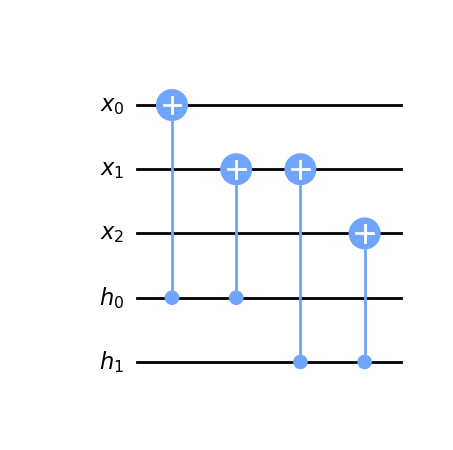
\includegraphics[scale=0.7]{26.png}
\end{center}
\subsection*{Exercise 10.27}
Consider a bit error $e_1$ and flip error $e_2$. We get,\\
$\displaystyle\frac{1}{\sqrt{|C_2|}}\sum_{y\in C_2}(-1)^{u.y}
(-1)^{(x+y+v).e_2}\ket{x+y+v+e_1}$\\
Applying the parity matrix $H_1$ to $\ket{x+C_2}\ket{0}$ we get,\\
$\displaystyle\frac{1}{\sqrt{|C_2|}}\sum_{y\in C_2}(-1)^{u.y}
(-1)^{(x+y+v).e_2}\ket{x+y+v}\ket{H_1(v+e_1)}$\\
As $v$ is known so is $H_1v$, hence we can calculate the syndrome
$H_1e_1$. Therefore, removing the bit error we get,\\
$\displaystyle\frac{1}{\sqrt{|C_2|}}\sum_{y\in C_2}(-1)^{u.y}
(-1)^{(x+y+v).e_2}\ket{x+y+v}$\\
Applying Hadamard gates to each qubit we get,\\
$\displaystyle\frac{1}{\sqrt{|C_2|2^n}}\sum_z\sum_{y\in C_2}
(-1)^{u.y}(-1)^{(x+y+v).(z+e_2)}\ket{z}=
\frac{1}{\sqrt{|C_2|2^n}}\sum_z\sum_{y\in C_2}
(-1)^{(u+z+e_2).y}(-1)^{(x+v).(z+e_2)}\ket{z}$\\
Let $e_2+z=z^\prime+u$, then we have,\\
$\displaystyle\frac{1}{\sqrt{|C_2|2^n}}\sum_{z^\prime}\sum_{y\in C_2}
(-1)^{z^\prime.y}(-1)^{(x+v).(z^\prime +u)}\ket{z^\prime+e_2+u}$\\
Using Exercise 10.25 we get,\\
$\displaystyle\frac{1}{\sqrt{2^n/|C_2|}}\sum_{z^\prime\in C_2^\perp}
(-1)^{(x+v).(z^\prime +u)}\ket{z^\prime+e_2+u}$\\
Once again by knowing $H_2u$ we calculate the syndrome $H_2e_2$, where
$H_2$ is the parity check matrix for $C_2^\perp$, and hence correct the
error $e_2$ to get,\\
$\displaystyle\frac{1}{\sqrt{2^n/|C_2|}}\sum_{z^\prime\in C_2^\perp}
(-1)^{(x+v).(z^\prime +u)}\ket{z^\prime+u}$\\
Applying the Hadamards again we get,\\
$\displaystyle\frac{1}{\sqrt{|C_2|}}\sum_{y\in C_2}(-1)^{u.y}
\ket{x+y+v}$\\
Hence, this has the same error-correcting properties as the
$CSS(C_1,C_2)$.
\subsection*{Exercise 10.28}
For the $[7,4,3]$ Hamming code we have,\\
$H=
\begin{bmatrix}
    0&0&0&1&1&1&1\\
    0&1&1&0&0&1&1\\
    1&0&1&0&1&0&1
\end{bmatrix}$\\
$HH[C_2]^T=\begin{bmatrix}
    0&0&0&1&1&1&1\\
    0&1&1&0&0&1&1\\
    1&0&1&0&1&0&1
\end{bmatrix}
\begin{bmatrix}
    1&0&0&0\\
    0&1&0&0\\
    0&0&1&0\\
    0&0&0&1\\
    0&1&1&1\\
    1&0&1&1\\
    1&1&0&1\\
\end{bmatrix}=
\begin{bmatrix}
    0&0&0&0\\
    0&0&0&0\\
    0&0&0&0
\end{bmatrix}$\\
Hence, $H[C_2]^T=G[C_1]$.
\subsection*{Exercise 10.29}
Let $\ket{x},\ket{y}\in V_S$, i.e. $\forall g\in S$ 
$g\ket{x}=\ket{x}$ and $g\ket{y}=\ket{y}$. Consider $a\ket{x}+b\ket{y}$
for some $a$ and $b$. As $g$ are linear operators we have,\\
$g(a\ket{x}+b\ket{y})=ag\ket{x}+bg\ket{y}=a\ket{x}+b\ket{y}$\\
Hence, $a\ket{x}+b\ket{y}\in V_S$.\\
Let $\ket{x}\in V_S\implies \forall g\in S$ $g\ket{x}=\ket{x}\implies \forall
g\in S$ $\ket{x}\in V_g\implies \ket{x}\in \displaystyle \bigcap_{g\in S}V_G$ 
\subsection*{Exercise 10.30}
Let $\pm iI\in S$ then as $S$ is a group $(\pm iI)(\pm iI)\in S$, hence $-I\in S$, which
is a contradiction therefore $\pm iI\notin S$.
\subsection*{Exercise 10.31}
If $g_i$ and $g_j$ commute then all the elements of $S$ commute, as
$S$ is generated by the $g_i$'s. If all the elements of $S$ commute
then necessarily $g_i$ and $g_j$ also commute as they're elements
of $S$.
\subsection*{Exercise 10.32}
$g_1\ket{0_L}=\frac{1}{\sqrt{8}}(\ket{0001111}+\ket{1011010}+
\ket{0111100}+\ket{1101001}+\ket{0000000}+\ket{1010101}
+\ket{0110011}+\ket{1100110})=\ket{0_L}$\\
Similarly, for $g_2$ and $g_3$.\\
For $g_3$ to $g_6$, each block has an even number of phase flips, hence
overall no overall phase flip takes place.\\
Similarly as above for the $\ket{1_L}$.
\subsection*{Exercise 10.33}
Let $r(g)=[\vec{x}|\vec{z}]$ and
$r(g^\prime)=[\vec{x}^\prime|\vec{z}^\prime]$. Then, \\
$r(g)\Lambda r(g^\prime)^T=\vec{x}.\vec{z^\prime}+
\vec{z}.\vec{x^\prime}$\\
If $g$ and $g^\prime$ commute then in total there are even number of
anti-commuting Pauli operators, hence the sum of the $2$ scalar products mod $2$
will be $0$. If $r(g)\Lambda r(g^\prime)^T=0$ then both scalar products will have to be $0$ or
$1$, hence there are an even number of anti-commuting Pauli operators, hence
$g$ and $g^\prime$ commute.
\subsection*{Exercise 10.34}
A counterexample is $S=<X, Z>$. $XZXZ=(-iY)(-iY)=-I$. 
\subsection*{Exercise 10.35}
Each $g$ is a tensor product of Pauli operators with prefactors
$\pm i$ or $\pm 1$, hence 
$g^2=\pm I$. However, $g^2\in S$, but $-I\notin S$, therefore
$g^2=I$.
\subsection*{Exercise 10.36}
$UX_2U^\dagger=
\begin{bmatrix}
I&0\\
0&X    
\end{bmatrix}
\begin{bmatrix}
    X&0\\
    0&X    
\end{bmatrix}
\begin{bmatrix}
    I&0\\
    0&X    
\end{bmatrix}=
\begin{bmatrix}
    I&0\\
    0&X    
\end{bmatrix}
\begin{bmatrix}
    X&0\\
    0&I    
\end{bmatrix}=
\begin{bmatrix}
    X&0\\
    0&X    
\end{bmatrix}=X_2$\\
$UZ_1U^\dagger=\begin{bmatrix}
    I&0\\
    0&X    
    \end{bmatrix}
    \begin{bmatrix}
        I&0\\
        0&-I    
    \end{bmatrix}
    \begin{bmatrix}
        I&0\\
        0&X    
    \end{bmatrix}=
    \begin{bmatrix}
        I&0\\
        0&X    
    \end{bmatrix}
    \begin{bmatrix}
        I&0\\
        0&-X    
    \end{bmatrix}=
    \begin{bmatrix}
        I&0\\
        0&-I    
    \end{bmatrix}=Z_1$\\
$UZ_2U^\dagger=\begin{bmatrix}
    I&0\\
    0&X    
    \end{bmatrix}
    \begin{bmatrix}
        Z&0\\
        0&Z    
    \end{bmatrix}
    \begin{bmatrix}
        I&0\\
        0&X    
    \end{bmatrix}=
    \begin{bmatrix}
        I&0\\
        0&X    
    \end{bmatrix}
    \begin{bmatrix}
        Z&0\\
        0&-iY    
    \end{bmatrix}=
    \begin{bmatrix}
        Z&0\\
        0&-Z    
    \end{bmatrix}=Z_1Z_2$
\subsection*{Exercise 10.37}
$UY_1U^\dagger=
\begin{bmatrix}
    I&0\\
    0&X    
    \end{bmatrix}
    \begin{bmatrix}
        0&-iI\\
        iI&0    
    \end{bmatrix}
    \begin{bmatrix}
        I&0\\
        0&X    
    \end{bmatrix}=
    \begin{bmatrix}
        I&0\\
        0&X    
    \end{bmatrix}
    \begin{bmatrix}
        0&-iX\\
        iI&0    
    \end{bmatrix}=
    \begin{bmatrix}
        0&-iX\\
        iX&0    
    \end{bmatrix}=Y_1X_2$
\subsection*{Exercise 10.38}
\subsection*{Exercise 10.39}
$SXS^\dagger=
\begin{bmatrix}
    1&0\\
    0&i
\end{bmatrix}
\begin{bmatrix}
    0&1\\
    1&0
\end{bmatrix}
\begin{bmatrix}
    1&0\\
    0&-i
\end{bmatrix}=
\begin{bmatrix}
    1&0\\
    0&i
\end{bmatrix}
\begin{bmatrix}
    0&-i\\
    1&0
\end{bmatrix}=
\begin{bmatrix}
    0&-i\\
    i&0
\end{bmatrix}=Y$\\
$SXS^\dagger=
\begin{bmatrix}
    1&0\\
    0&i
\end{bmatrix}
\begin{bmatrix}
    1&0\\
    0&-1
\end{bmatrix}
\begin{bmatrix}
    1&0\\
    0&-i
\end{bmatrix}=
\begin{bmatrix}
    1&0\\
    0&i
\end{bmatrix}
\begin{bmatrix}
    1&0\\
    0&i
\end{bmatrix}=
\begin{bmatrix}
    1&0\\
    1&-1
\end{bmatrix}=Z$
\subsection*{Exercise 10.40}
1) First, consider $UZU^\dagger=Z$, for this to be true
we require $U=\begin{bmatrix}
    1&0\\
    0&e^{i\phi}
\end{bmatrix}$. For this $U$ we see that, 
$UXU^\dagger=\pm X, \pm Y$, with $e^{i\phi}=\pm 1, \pm i$.
Therefore, we see that $U$ can be constructed using only phase gates.\\
From Chapter 4 we know that for and Pauli operator $\sigma$ there exists
$R$ constructed from Hadamards and phase gates, such that
$R\sigma R^\dagger =Z$.\\
Let's consider a normalizer $U$ for $G_1$. Then, $\exists g\in G_1$ such
that $UgU^\dagger=Z$. Let $U=VR$, where $R$ is defined as above.
Then, $UgU^\dagger=VRgR^\dagger V^\dagger=VZV^\dagger=Z$, hence from above
$V$ consists of only phase gates and $R$ consists of phase and Hadamard gates, therefore
$U$ consists of only phase and Hadamard gates.\\
Therefore, phase and Hadamard gates can be used to construct any normalizer one
$G_1$.\\
2) Let the process described by the circuit be $\bar{U}$. We like to show
$\bra{a}\bar{U}\ket{b}\ket{\psi}=\bra{a}U\ket{b}\ket{\psi}$ $\forall a,b,\psi$.\\
First we get the following from the conditions on $U$,\\
$UZ_1=(X_1\otimes g)U$\\
$X_1U=(I\otimes g)UZ_1=gUZ_1$\\
$UX_1=(Z_1\otimes g^\prime)U$\\
$Z_1U=(I\otimes g^\prime)UX_1=g^\prime UX_1$\\
Now consider $U^\prime\ket{\psi}$\\
$U^\prime\ket{\psi}=\sqrt{2}\bra{0}U(\ket{0}\ket{\psi})=
\sqrt{2}\bra{0}X_1gUZ_1(\ket{0}\ket{\psi})=
\sqrt{2}\bra{1}gU(\ket{0}\ket{\psi})$\\
$U^\prime\ket{\psi}=\sqrt{2}\bra{0}Z_1g^\prime UX_1(\ket{0}\ket{\psi})=
\sqrt{2}\bra{0}g^\prime U(\ket{1}\ket{\psi})$\\
$U^\prime\ket{\psi}=\sqrt{2}\bra{1}Z_1g g^\prime UX_1(\ket{0}\ket{\psi})
-\sqrt{2}\bra{1}g g^\prime U(\ket{1}\ket{\psi})$\\
Now consider, $\bra{a}\bar{U}\ket{b}\ket{\psi}$.\\
$\bra{0}\bar{U}\ket{0}\ket{\psi}=\bra{0}\frac{1}{\sqrt{2}}
(\ket{0}\otimes U^\prime \ket{\psi}+\ket{1}\otimes gU^\prime\ket{\psi})=
\frac{1}{\sqrt{2}}U^\prime\ket{\psi}=\bra{0}U\ket{0}\ket{\psi}$\\
$\bra{0}\bar{U}\ket{1}\ket{\psi}=\bra{0}\frac{1}{\sqrt{2}}
(\ket{0}\otimes g^\prime U^\prime \ket{\psi}-\ket{1}\otimes gg^\prime U^\prime\ket{\psi})=
\frac{1}{\sqrt{2}}g^\prime U^\prime\ket{\psi}=\bra{0}U\ket{1}\ket{\psi}$\\
$\bra{1}\bar{U}\ket{1}\ket{\psi}=\bra{1}\frac{1}{\sqrt{2}}
(\ket{0}\otimes g^\prime U^\prime \ket{\psi}-\ket{1}\otimes gg^\prime U^\prime\ket{\psi})=
-\frac{1}{\sqrt{2}}gg^\prime U^\prime\ket{\psi}=-\bra{1}U\ket{1}\ket{\psi}$\\
$\bra{1}\bar{U}\ket{0}\ket{\psi}=\bra{1}\frac{1}{\sqrt{2}}
(\ket{0}\otimes U^\prime \ket{\psi}+\ket{1}\otimes gU^\prime\ket{\psi})=
\frac{1}{\sqrt{2}}gU^\prime\ket{\psi}=\bra{1}U\ket{0}\ket{\psi}$\\
Hence, $\bra{a}\bar{U}\ket{b}\ket{\psi}=\bra{a}U\ket{b}\ket{\psi}$ $\forall a,b,\psi$, therefore
$U=\bar{U}$.\\
Overall, $U$ is composed of $U^\prime$ and $O(n)$ phase and Hadamard
gates. As construction of a gate $U\in N(G_{n+1})$ requires a gate
$U^\prime \in N(G_n)$, for gate $U$ we need $\displaystyle\sum_{i=1}^nO(i)=O(n^2)$ phase and
Hadamard gates.\\
3) Consider $UZ_1U^\dagger = g$ and $UX_1U^\dagger=g^\prime$. Then 
$\{g,g^\dagger\}=0$ as $\{Z_1,X_1\}=0$. Hence, $g$ and $g^\prime$ have at
some position $j$ $\sigma_j\neq\sigma_j^\prime$. Hence, we use the SWAP operator to turn the
situation of that of part (2).\\
$\textbf{SWAP}_{1j}UZ_1U^\dagger\textbf{SWAP}_{1j}^\dagger=\sigma\otimes g_1$\\
$\textbf{SWAP}_{1j}UX_1U^\dagger\textbf{SWAP}_{1j}^\dagger=\sigma^\prime\otimes g_1^\prime$\\
As we can construct pauli operators using Hadamard and phase gates,
if $\sigma\neq\sigma^\prime$ then $R\sigma R^\dagger=Z_1$ and $R\sigma^\prime R^\dagger=X_1$
for some $R$ constructed from phase and Hadamard gates. Then,\\
$R\textbf{SWAP}_{1j}UZ_1U^\dagger\textbf{SWAP}_{1j}^\dagger R^\dagger=Z_1\otimes g_1$\\
$R\textbf{SWAP}_{1j}UZ_1U^\dagger\textbf{SWAP}_{1j}^\dagger R^\dagger=X_1\otimes g_1$\\
which is the situation of part (2).\\
Therefore, as the \textbf{SWAP} is made out of 3 \textbf{CNOT}s, we conclude
that any normalizer can be written as a composition of $O(n^2)$ phase, Hadamard and
\textbf{CNOT} gates.
\subsection*{Exercise 10.41}
$T=\begin{bmatrix}
    1&0\\
    0&e^{i\pi/4}
\end{bmatrix}$\\
$TZT^\dagger=\begin{bmatrix}
    1&0\\
    0&e^{i\pi/4}
\end{bmatrix}
\begin{bmatrix}
    1&0\\
    0&-1
\end{bmatrix}
\begin{bmatrix}
    1&0\\
    0&e^{-i\pi/4}
\end{bmatrix}=
\begin{bmatrix}
    1&0\\
    0&-e^{i\pi/4}e^{-i\pi/4}
\end{bmatrix}=Z$\\
$TXT^\dagger=\begin{bmatrix}
    1&0\\
    0&e^{i\pi/4}
\end{bmatrix}
\begin{bmatrix}
    0&1\\
    1&0
\end{bmatrix}
\begin{bmatrix}
    1&0\\
    0&e^{-i\pi/4}
\end{bmatrix}=
\begin{bmatrix}
    1&0\\
    0&e^{i\pi/4}
\end{bmatrix}
\begin{bmatrix}
    0&e^{-i\pi/4}\\
    1&0
\end{bmatrix}=
\begin{bmatrix}
    0&e^{-i\pi/4}\\
    e^{i\pi/4}&0
\end{bmatrix}=
\begin{bmatrix}
    0&\frac{1-i}{\sqrt{2}}\\
    \frac{1+i}{\sqrt{2}}&0
\end{bmatrix}=\frac{X+Y}{\sqrt{2}}$\\
$U=\begin{bmatrix}
    I&0&0&0\\
    0&I&0&0\\
    0&0&I&0\\
    0&0&0&X
\end{bmatrix}$\\
$UZ_1U^\dagger=\begin{bmatrix}
    I&0&0&0\\
    0&I&0&0\\
    0&0&I&0\\
    0&0&0&X
\end{bmatrix}
\begin{bmatrix}
    I&0&0&0\\
    0&I&0&0\\
    0&0&-I&0\\
    0&0&0&-I
\end{bmatrix}
\begin{bmatrix}
    I&0&0&0\\
    0&I&0&0\\
    0&0&I&0\\
    0&0&0&X
\end{bmatrix}=
\begin{bmatrix}
    I&0&0&0\\
    0&I&0&0\\
    0&0&-I&0\\
    0&0&0&-XX
\end{bmatrix}=Z_1$
$UZ_2U^\dagger=\begin{bmatrix}
    I&0&0&0\\
    0&I&0&0\\
    0&0&I&0\\
    0&0&0&X
\end{bmatrix}
\begin{bmatrix}
    I&0&0&0\\
    0&-I&0&0\\
    0&0&I&0\\
    0&0&0&-I
\end{bmatrix}
\begin{bmatrix}
    I&0&0&0\\
    0&I&0&0\\
    0&0&I&0\\
    0&0&0&X
\end{bmatrix}=
\begin{bmatrix}
    I&0&0&0\\
    0&-I&0&0\\
    0&0&I&0\\
    0&0&0&-XX
\end{bmatrix}=Z_2$
$UX_3U^\dagger=\begin{bmatrix}
    I&0&0&0\\
    0&I&0&0\\
    0&0&I&0\\
    0&0&0&X
\end{bmatrix}
\begin{bmatrix}
    X&0&0&0\\
    0&X&0&0\\
    0&0&X&0\\
    0&0&0&X
\end{bmatrix}
\begin{bmatrix}
    I&0&0&0\\
    0&I&0&0\\
    0&0&I&0\\
    0&0&0&X
\end{bmatrix}=
\begin{bmatrix}
    X&0&0&0\\
    0&X&0&0\\
    0&0&X&0\\
    0&0&0&XXX
\end{bmatrix}=X_3$\\
$UX_1U^\dagger=\begin{bmatrix}
    I&0&0&0\\
    0&I&0&0\\
    0&0&I&0\\
    0&0&0&X
\end{bmatrix}
\begin{bmatrix}
    0&0&I&0\\
    0&0&0&I\\
    I&0&0&0\\
    0&I&0&0
\end{bmatrix}
\begin{bmatrix}
    I&0&0&0\\
    0&I&0&0\\
    0&0&I&0\\
    0&0&0&X
\end{bmatrix}=
\begin{bmatrix}
    I&0&0&0\\
    0&I&0&0\\
    0&0&I&0\\
    0&0&0&X
\end{bmatrix}
\begin{bmatrix}
    0&0&I&0\\
    0&0&0&X\\
    I&0&0&0\\
    0&I&0&0
\end{bmatrix}=
\begin{bmatrix}
    0&0&I&0\\
    0&0&0&X\\
    I&0&0&0\\
    0&X&0&0
\end{bmatrix}=X_1\otimes
\begin{bmatrix}
    I&0\\
    0&X
\end{bmatrix}=X_1\otimes
\frac{
    \begin{bmatrix}
        I&0\\
        0&I
    \end{bmatrix}+
    \begin{bmatrix}
        I&0\\
        0&-I
    \end{bmatrix}+
    \begin{bmatrix}
        X&0\\
        0&X
    \end{bmatrix}+
    \begin{bmatrix}
        -X&0\\
        0&X
    \end{bmatrix}
}{2}=\\
\displaystyle X_1\otimes\frac{I+Z_2+X_3-Z_2X_3}{2}$\\
$UX_2U^\dagger=\begin{bmatrix}
    I&0&0&0\\
    0&I&0&0\\
    0&0&I&0\\
    0&0&0&X
\end{bmatrix}
\begin{bmatrix}
    0&I&0&0\\
    I&0&0&0\\
    0&0&0&I\\
    0&0&I&0
\end{bmatrix}
\begin{bmatrix}
    I&0&0&0\\
    0&I&0&0\\
    0&0&I&0\\
    0&0&0&X
\end{bmatrix}=
\begin{bmatrix}
    I&0&0&0\\
    0&I&0&0\\
    0&0&I&0\\
    0&0&0&X
\end{bmatrix}
\begin{bmatrix}
    0&I&0&0\\
    I&0&0&0\\
    0&0&0&X\\
    0&0&I&0
\end{bmatrix}=
\begin{bmatrix}
    0&I&0&0\\
    I&0&0&0\\
    0&0&0&X\\
    0&0&X&0
\end{bmatrix}=\frac{1}{2}\left\{
\begin{bmatrix}
    0&I&0&0\\
    I&0&0&0\\
    0&0&0&I\\
    0&0&I&0
\end{bmatrix}+
\begin{bmatrix}
    0&I&0&0\\
    I&0&0&0\\
    0&0&0&-I\\
    0&0&-I&0
\end{bmatrix}+
\begin{bmatrix}
    0&X&0&0\\
    X&0&0&0\\
    0&0&0&X\\
    0&0&X&0
\end{bmatrix}+
\begin{bmatrix}
    0&-X&0&0\\
    -X&0&0&0\\
    0&0&0&X\\
    0&0&X&0
\end{bmatrix}
\right\}\\
=\displaystyle X_2\otimes\frac{I+Z_1+X_3-Z_1X_3}{2}$\\
$UZ_3U^\dagger=\begin{bmatrix}
    I&0&0&0\\
    0&I&0&0\\
    0&0&I&0\\
    0&0&0&X
\end{bmatrix}
\begin{bmatrix}
    Z&0&0&0\\
    0&Z&0&0\\
    0&0&Z&0\\
    0&0&0&Z
\end{bmatrix}
\begin{bmatrix}
    I&0&0&0\\
    0&I&0&0\\
    0&0&I&0\\
    0&0&0&X
\end{bmatrix}=
\begin{bmatrix}
    Z&0&0&0\\
    0&Z&0&0\\
    0&0&Z&0\\
    0&0&0&XZX
\end{bmatrix}=
\begin{bmatrix}
    Z&0&0&0\\
    0&Z&0&0\\
    0&0&Z&0\\
    0&0&0&-Z
\end{bmatrix}=\frac{1}{2}\left\{
    \begin{bmatrix}
        Z&0&0&0\\
        0&Z&0&0\\
        0&0&Z&0\\
        0&0&0&Z
    \end{bmatrix}+
    \begin{bmatrix}
        Z&0&0&0\\
        0&Z&0&0\\
        0&0&-Z&0\\
        0&0&0&-Z
    \end{bmatrix}+
    \begin{bmatrix}
        Z&0&0&0\\
        0&-Z&0&0\\
        0&0&Z&0\\
        0&0&0&-Z
    \end{bmatrix}+
    \begin{bmatrix}
        -Z&0&0&0\\
        0&Z&0&0\\
        0&0&Z&0\\
        0&0&0&-Z
    \end{bmatrix}
\right\}\\
=\displaystyle Z_3\otimes\frac{I+Z_1+Z_2-Z_1Z_2}{2}$
\subsection*{Exercise 10.42}
Initially $S=<IXX,IZZ>$ with $\bar{Z}=ZII$ and $\bar{X}=XII$.
Considering the effect of the circuit on the generators we get,\\
$IXX\xrightarrow{CNOT}IXX\xrightarrow{H}IXX
\xrightarrow{\text{Mes. }X_1}IXX
\xrightarrow{\text{Mes. }Z_2}IZI$\\
$IZZ\xrightarrow{CNOT}ZZZ\xrightarrow{H}XZZ
\xrightarrow{\text{Mes. }X_1}XZZ
\xrightarrow{\text{Mes. }Z_2}XZZ$\\
For the final $S_f=<IZI,XZZ>$ we have $\bar{Z}=IIZ$ and $\bar{X}=IIX$,
hence the circuit does indeed teleport the initial state.
\subsection*{Exercise 10.43}
$\forall g \in S$ we have $g\in N(S)$ as $gg^\prime g^\dagger \in S$ $\forall g^\prime\in S$ due to
$S$ being a group. Therefore, $S\subseteq N(S)$.
\subsection*{Exercise 10.44}
\subsection*{Exercise 10.45}

\subsection*{Exercise 10.46}
$S=<X_1X_2,X_2X_3>=\{I,X_1X_2,X_2X_3,X_1X_3\}$\\
The subspace fixed by $X_1X_2$ is spanned by $\ket{+++},\ket{++-},\ket{---}$ and $\ket{--+}$.
The subspace fixed by $X_2X_3$ is spanned by $\ket{+++},\ket{-++},\ket{---}$ and $\ket{-++}$.
Hence, the subspace fixed by $S$ is spanned by $\ket{+++}$ and $\ket{---}$, which is the subspace
for the three qubit phase flip code. Therefore, $X_1X_2$ and $X_2X_3$ generate the stabilizer
for the three qubit phase flip code. 
\subsection*{Exercise 10.47}
The generators 1-6 have 2 $Z$'s with both $Z$'s being in one of the triplets,
hence the phase flips are cancelled and $\ket{0_L}$ and $\ket{1_L}$ are fixed by them.\\
Generators 7 and 8 have $X$s on all elements of any of the triplets or none. Hence, they fix
$\ket{0_L}$. As 2 triplets are acted on, the phase flip from the triplets is cancelled and 
hence $\ket{1_L}$ is also fixed. Therefore, theses are the generators for the Shor-code.
\subsection*{Exercise 10.48}
Each generator has an even number of $Z$'s or $X$'s, hence commute with $\bar{Z}$ and $\bar{X}$.
Counting $Y$'s as both an $X$ and a $Z$, any product of the generators has an even number of $Z$'s
and an even number of $X$'s, therefore as $\bar{Z}$ has an odd number of $Z$'s and
$\bar{X}$ has an odd number of $X$'s they are independent of the generators. Lastly,
$\bar{X}\bar{Z}=(XZ)^{\otimes 9}=(-1)^9(ZX)^{\otimes 9}=-\bar{Z}\bar{X}$. Therefore,
$\bar{Z}$ and $\bar{X}$ act as logical $Z$ and $X$ operators for the Shor-code.
\subsection*{Exercise 10.49}
Consider the set $E=\{X_1,\ldots X_5,Y_1\ldots Y_5, Z_1,\ldots Z_5\}$.
Consider for example the combination $X_1Z_2$. It commutes with $g_2$ hence $X_1Z_2\notin N(S)$.
Similarly, we can show that $\forall E_iE_j$, $E_iE_j\notin N(S)$ or $E_iE_j\in S$, and hence
$E_iE_j\notin N(S)-S$, therefore by Theorem 10.8 the five qubit code can protect against an
arbitrary single qubit error. 
\subsection*{Exercise 10.50}
For the five qubit code $t=1$, $n=5$ and $k=1$. Hence, the Hamming bound is\\
$\displaystyle{5\choose 0}3^02^1+{5\choose 1}3^12^1=2+5\times 6=32=2^5$\\
Therefore, the five qubit code saturates the Hamming bound.
\subsection*{Exercise 10.51}
The given check matrix is split into generators with only $X$'s and generators only into $Z$'s.
Consider the set $E$ of all possible $t$ operator tensor products of $X$'s and $Z$'s. Consider
$E_iE_j$. As both $C_1$ and $C_2$ correct up to $t$ errors, $\exists g\in S$ such that 
for the $2t$ length row $E_iE_j$ $E_iE_jgE_iE_j\notin S$ or $E_iE_j\in S$. Hence,
$E_iE_j\notin N(S)-S$, therefore, by Theorem 10.8 $E$ is a length $t$ set of correctable errors.
\subsection*{Exercise 10.52}
Using figure 10.6 for the stabilizers. Each generator has an even number of $Z$'s or
$X$'s, hence commute with $\bar{Z}$ and $\bar{X}$. 
Counting $Y$'s as both an $X$ and a $Z$, any product of the generators has an even number of $Z$'s
and an even number of $X$'s, therefore as $\bar{Z}$ has an odd number of $Z$'s and
$\bar{X}$ has an odd number of $X$'s they are independent of the generators. Lastly,
$\bar{X}\bar{Z}=(XZ)^{\otimes 7}=(-1)^7(ZX)^{\otimes 7}=-\bar{Z}\bar{X}$. Therefore,
$\bar{Z}$ and $\bar{X}$ act as logical $Z$ and $X$ operators for the Steane-code.
\subsection*{Exercise 10.53}
\subsection*{Exercise 10.54}
\subsection*{Exercise 10.55}
\subsection*{Exercise 10.56}
\subsection*{Exercise 10.57}
\subsection*{Exercise 10.58}
\subsection*{Exercise 10.59}
\subsection*{Exercise 10.60}
\subsection*{Exercise 10.61}
\subsection*{Exercise 10.62}
\subsection*{Exercise 10.63}
\subsection*{Exercise 10.64}
\subsection*{Exercise 10.65}
\subsection*{Exercise 10.66}
\subsection*{Exercise 10.67}
\subsection*{Exercise 10.68}
\subsection*{Exercise 10.69}

\end{document}